\chapter{Methods}\label{ch:methods}
This chapter introduces the different methods used to quantify uncertainty for curved surfaces from partial point clouds without any extra information available. We can formulate our task in two different scenarios regarding the availability of additional data or prior information related to the 3D shape. In case of prior knowledge or additional data being unavailable, we can only use the point cloud collected from multiple scans of the object. Then our task can be defined as:
\begin{problemnotitle}{SingleCloud}{}
    \probleminput{A point cloud with $N_C$ points represented by $\mathbf{X}=\left\{\mathbf{x}_{i} \in \mathbb{R}^{3}\right\}_{i=1}^{N_C}$.}
    \problemoutput{A probabilistic estimate of the distance from the surface or probability of lying on the surface for any point $\mathbf{x} \in \mathbb{R}^{3}$.}
\end{problemnotitle}
\newline

On the other hand, if we assume that we know the kind of object the 3D shape belongs to, we can use an additional dataset of related 3D shapes with partial and complete point clouds. Then for a dataset of partial point clouds $\mathbf{X_P} \in \mathbb{R}^{N \times N_P \times 3}$ with $N$ instances of $N_P$ points in each incomplete point cloud instance, we have a corresponding dataset of complete point clouds $\mathbf{X_C} \in \mathbb{R}^{N \times N_C \times 3}$ with $N$ instances of $N_C$ points in each ground truth complete point cloud instance. Then the problem statement becomes:
\begin{problemnotitle}{DataCloud}{}
    \probleminput{A partial point cloud with $N_P$ points represented by $\mathbf{X}=\left\{\mathbf{x}_{i} \in \mathbb{R}^{3}\right\}_{i=1}^{N_P}$.}
    \problemoutput{A probabilistic estimate of the distance from the surface or probability of lying on the surface for any point $\mathbf{x} \in \mathbb{R}^{3}$.}
\end{problemnotitle}
\newline

We can then use the learned distribution over the distance field or the probabilistic surface reconstruction for further downstream tasks.


\section{Empirical Uncertainty Quantification for Point Cloud Completion}\label{euqpcc}
In this section, we propose to solve the Problem~\ref{DataCloud} utilizing a point cloud completion method for the given input partial cloud. Instead of directly computing the probabilistic estimate of the underlying surface, we first generate multiple possible completions from the input and then empirically estimate the surface along with the associated uncertainty by matching points between generated complete clouds. We denote the partial cloud by $\tilde{X}=\left\{\mathbf{\tilde{x}}_{i} \in \mathbb{R}^{3}\right\}_{i=1}^{N_P}$ and the generated complete cloud by $\hat{X}=\left\{\mathbf{\hat{x}}_{i} \in \mathbb{R}^{3}\right\}_{i=1}^{N_C}$. So we aim to learn $p(\hat{X}|\tilde{X})$. During training, we also have access to the ground truth complete cloud, which we denote by $X=\left\{\mathbf{x}_{i} \in \mathbb{R}^{3}\right\}_{i=1}^{N_C}$. Since for any partial cloud, there are many possible complete clouds consistent with the partial cloud, we need to learn to generate non-deterministic predictions depending upon some source of randomness. In Chapter~\ref{ch:background}, we reviewed different ways to quantify uncertainty in deep learning models, which gives us an idea about how we can also implement similar methods to generate different predictions with randomness. But first, we will describe the standard architecture used for point completion.


    \subsection{General Structure of Point Completion Network}
    \begin{figure}[htb]
      \begin{center}
      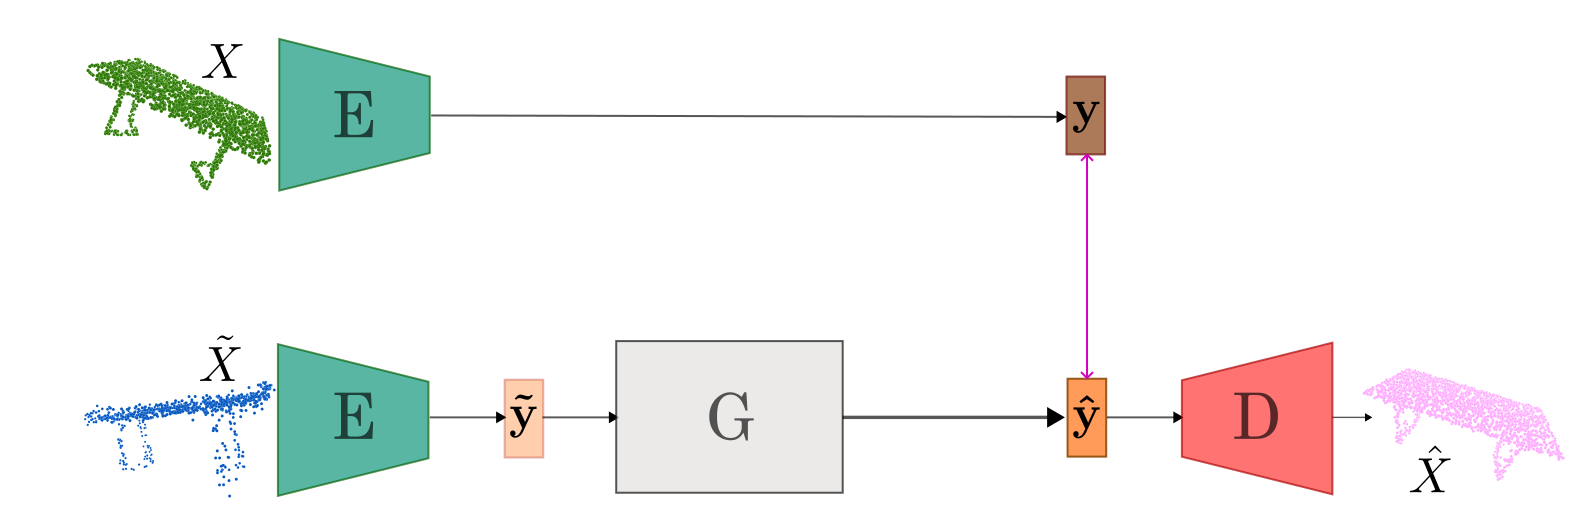
\includegraphics[width=\linewidth]{figures/general_network.png}
      \end{center}
      \caption{General structure of network used for training point cloud completion. During training, ground truth complete cloud $X$ is input to the encoder E to output the encoding $\mathbf{y}$. Parallelly partial cloud $\tilde{X}$ is input to the encoder E to generate the encoding $\mathbf{\tilde{y}}$, which is then given to generator G outputting new encoding $\mathbf{\hat{y}}$ which is compared to $\mathbf{y}$. The decoder D, on the other hand, produces a complete cloud $\hat{X}$ from  $\mathbf{\hat{y}}$.}\label{fig:gen_net}
    \end{figure}
    The general structure of our network used for point cloud completion consists of an auto-encoder (encoder-decoder network) and a generator network. We denote the encoder by E, decoder by D, and the generator by G (see Figure~\ref{fig:gen_net}). Via the auto-encoder network's encoder, we encode the partial shape represented by $\tilde{X}$ and the complete shape represented by $X$ to get the encodings $\mathbf{\tilde{y}}$ and $\mathbf{y}$ respectively. 
    \\
    Meanwhile, generator G generates a new encoding $\mathbf{\hat{y}}$ from the partial shape encoding $\mathbf{\tilde{y}}$ from which the decoder can produce a new complete shape $\hat{X}$. Generator G plays the role of the network, which incorporates the randomness of the completion method, since through G, we can generate different encodings from the partial cloud encoding. We can then produce different complete clouds via the decoder and empirically estimate the uncertainty of our completion method from the generated clouds. In the following section, we will describe how we can implement the above idea.

    
    \subsection{Uncertainty in Encoding Generation}
        \subsubsection{MC Dropout or DropConnect in Generator}
        \begin{figure}[htb]
          \begin{center}
          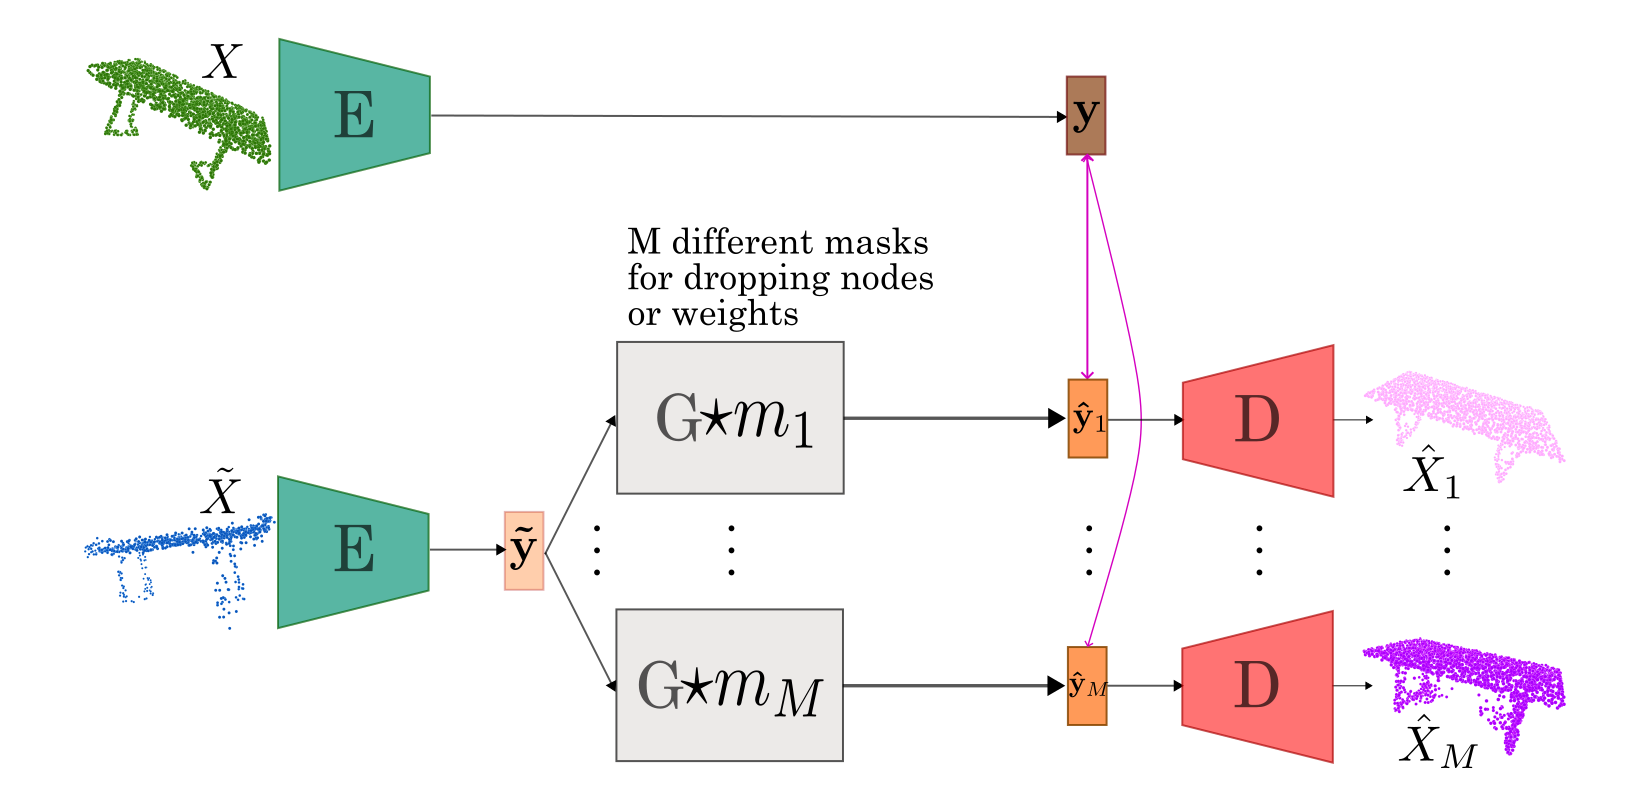
\includegraphics[width=\linewidth]{figures/drop_network.png}
          \end{center}
      \caption{Network for point cloud completion uncertainty quantification using dropout or DropConnect. During inference, the original generator network is modified based on some masking ($\{m_i\}_{i=1}^M$) multiple times to produce different generators.}\label{fig:drop_net}
        \end{figure}
        One simple idea to generate different encodings via the generator is to use dropout or DropConnect in the generator network while training. As explained in section~\ref{MCDrop}, we can also use dropout or DropConnect during inference to generate different encodings and complete shapes corresponding to those encodings for a particular input partial cloud (see Figure~\ref{fig:drop_net}). 
        
        \subsubsection{Deep Ensemble of Generators}
        \begin{figure}[htb]
          \begin{center}
          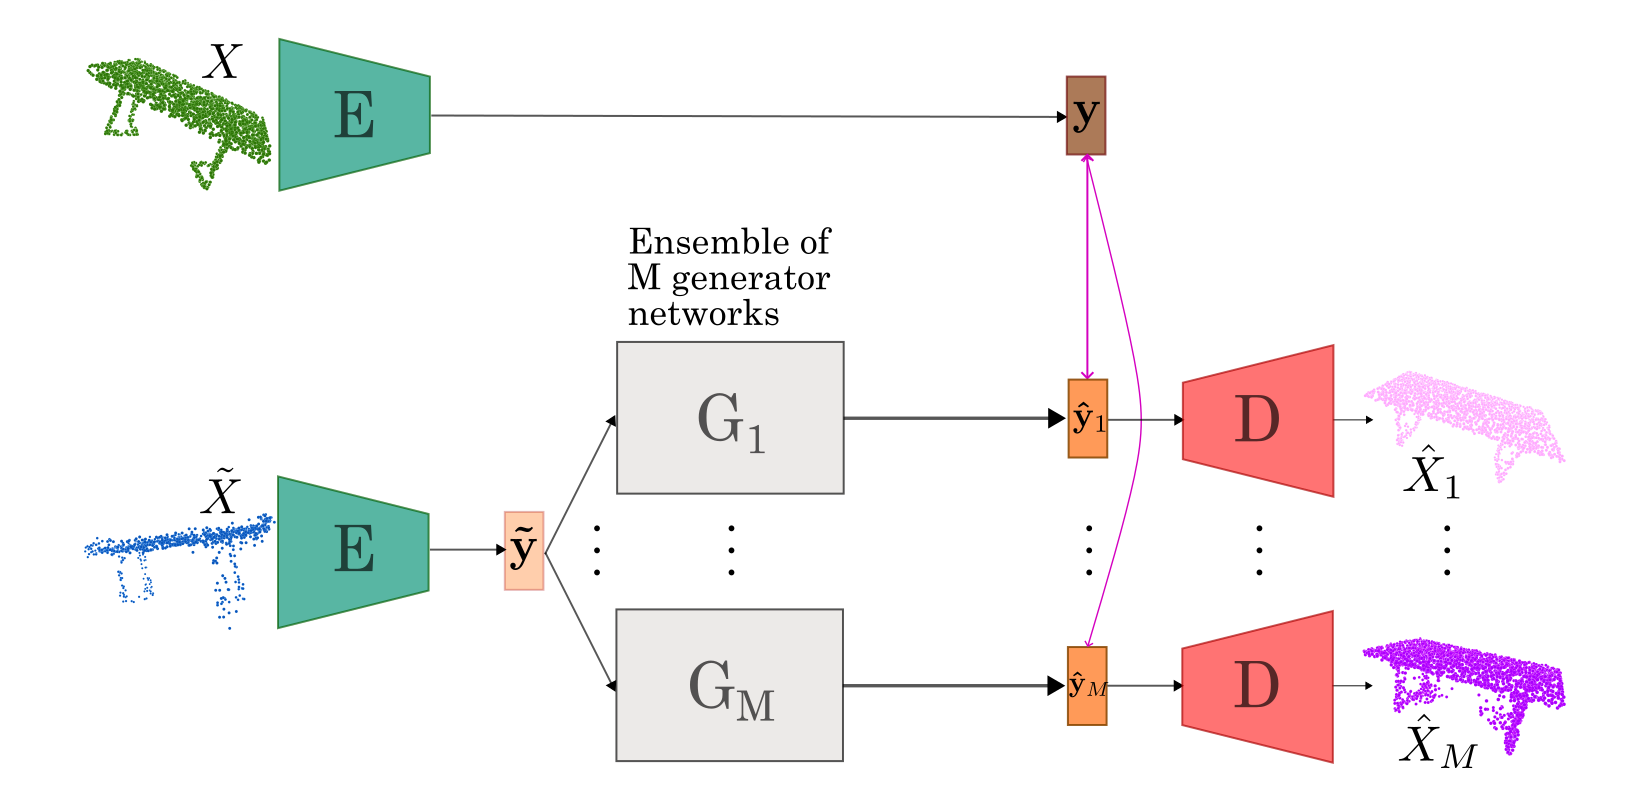
\includegraphics[width=\linewidth]{figures/ensemble_network.png}
          \end{center}
          \caption{Network for point cloud completion uncertainty quantification using deep ensemble. Different generators (based on the ensemble construction strategy) are trained. During inference, different generators produce different encodings.}\label{fig:ens_net}
        \end{figure}
        We can also use an ensemble of generators to train the point completion network. As described in section~\ref{Deepsemble}, there are many ways to construct the ensemble of generators. We will mostly focus on different initializations of parameters to create the ensemble. During inference, each generator in the ensemble outputs a different encoding, giving us different complete shapes(see Figure~\ref{fig:ens_net}).

        \subsubsection{Conditional Implicit Generative Model}
        \begin{figure}[htb]
          \begin{center}
          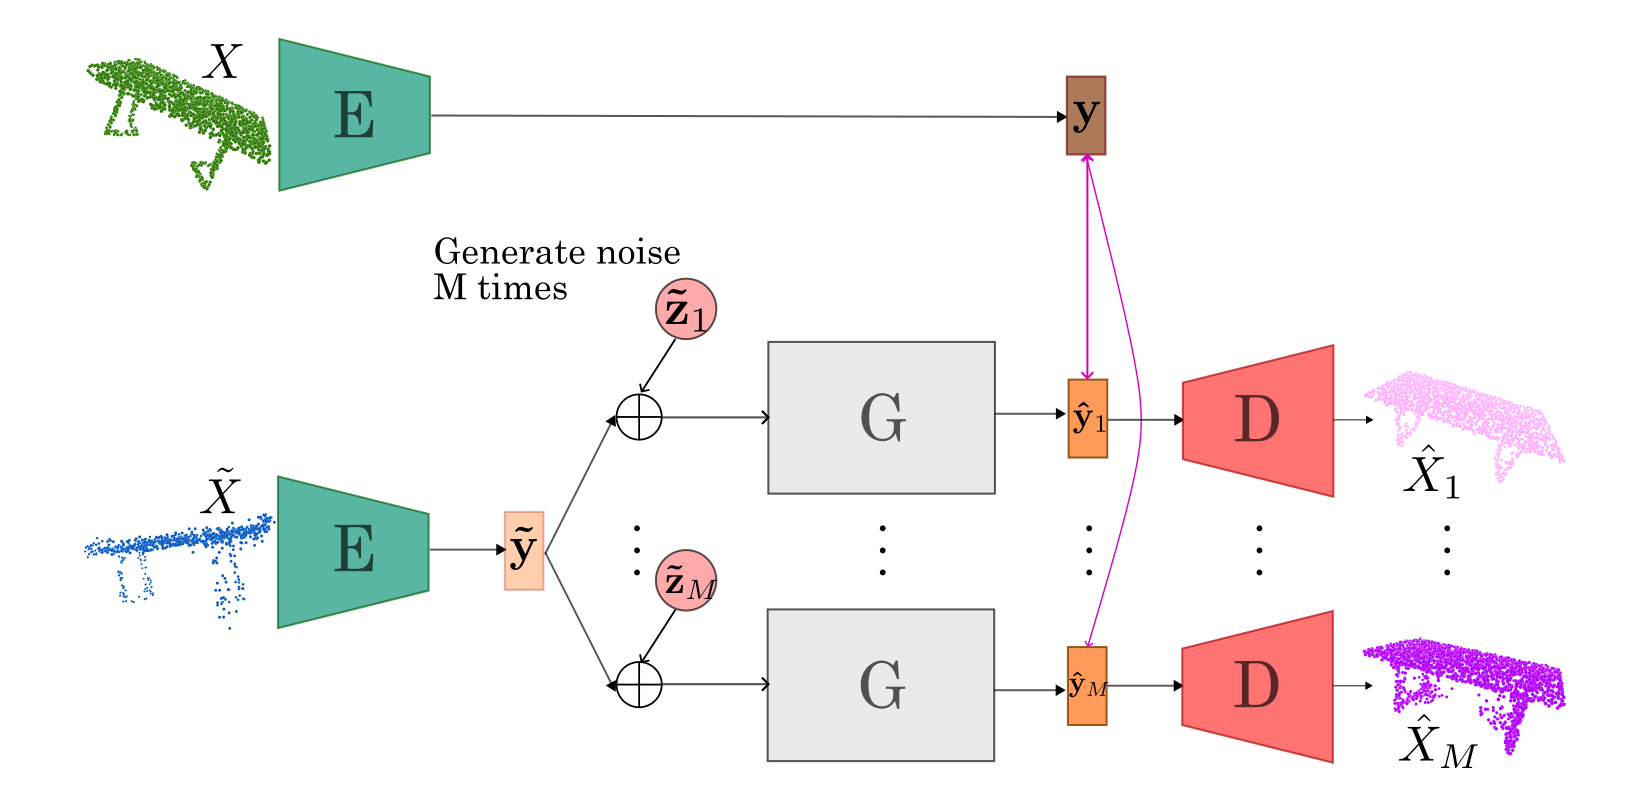
\includegraphics[width=\linewidth]{figures/implicit_gen_network.png}
          \end{center}
          \caption{Network for point cloud completion uncertainty quantification using conditional implicit generation. During inference, we sample noise from a standard Gaussian distribution multiple times and generate encodings based on the different noises.}\label{fig:implicit_net}
        \end{figure}
        Another possible method to generate non-deterministic predictions from an input is to add random noise to the input before passing it to the generator. We can reformulate Eq.~\ref{IGM} for conditional implicit generative models as:
        \begin{equation}\label{IGM}
            \mathbf{\tilde{z}} \sim q(\mathbf{z}), \quad \mathbf{\hat{y}} =  \mathcal{G}_\theta(\mathbf{\tilde{z}}; \mathbf{\tilde{y}})
        \end{equation}
        where $\mathcal{G}$ is specified by an NN with parameters $\theta$. With different $\mathbf{\tilde{z}}$ we can generate different $\mathbf{\hat{y}}$ corresponding to different complete shape for a fixed $\mathbf{\tilde{y}}$ (see Figure~\ref{fig:implicit_net}).

    \subsection{Training Procedure}
        \subsubsection{Learning encoding for point clouds}
        \begin{figure}[htb]
          \begin{center}
          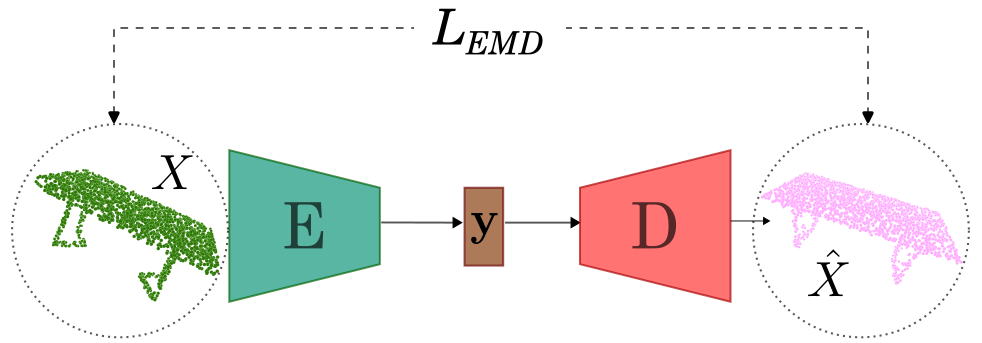
\includegraphics[width=\linewidth]{figures/emd_ae.png}
          \end{center}
          \caption{Training autoencoder by minimizing Earth mover's distance.}\label{fig:emd_ae}
        \end{figure}
        We learn to produce the encoding of a given point cloud by training an autoencoder, which encodes the given input to a lower-dimensional feature vector called a latent code or an encoding, and subsequently decodes the encoding to reconstruct the original input. The auto-encoder can be a standard auto-encoder (AE), a variational auto-encoder (VAE), or a vector-quantized variational auto-encoder (VQ-VAE), according to our deliberate choice. So, our auto-encoder is trained for a reconstruction task on a point cloud dataset for both partial and complete shapes.
        \newline
        
        For instances of ground truth point cloud $X=\left\{\mathbf{x}_{i} \in \mathbb{R}^{3}\right\}_{i=1}^{N_C}$ from the dataset of complete clouds $\mathbf{X_C} \in \mathbb{R}^{N \times N_C \times 3}$, we train an encoder-decoder network to learn an encoder mapping $\mathcal{E}: \mathbb{R}^{N_C \times 3} \rightarrow \mathbb{R}^{\ell}$ that takes the concatenation of coordinates of the $N_C$ points in complete cloud as input and produces an encoding in the latent space with dimension $\ell$ along with a decoder mapping $\mathcal{D}: \mathbb{R}^{\ell} \rightarrow \mathbb{R}^{N_C \times 3}$ that inverts the encoding back to a reconstructed point cloud with $N_C$ points as before. The autoencoder is trained using a reconstruction loss based on Earth Mover's Distance (EMD). The reconstruction loss for a point cloud $X$ is denoted as:
        \begin{equation}\label{emd_loss}
            L_{EMD} = d_{EMD}\left(X, \mathcal{D}(\mathcal{E}(X))\right),
        \end{equation}
        where $d_{EMD}\left(X, \mathcal{D}(\mathcal{E}(X))\right)$ denotes the Earth Mover's Distance between the input cloud and the reconstructed cloud (see Figure~\ref{fig:emd_ae}). We can then compute the objective function for training the autoencoder as:
        \begin{equation}\label{emd_obj}
            \mathcal{L}_{EMD} = \mathbb{E}_{X \sim p(X)} \left[d_{EMD}\left(X, \mathcal{D}(\mathcal{E}(X))\right)\right]
        \end{equation}
        where $p(X)$ denotes a distribution over the space of complete clouds from which we sample.
        \newline
        
        The encoding produced by the encoder provides a ready-made representation, which implicitly captures the shape manifold for a point cloud, to be used in downstream tasks. So, once training is done, we fix the network parameters while using the encoder and decoder in any subsequent network. As for the instances of point cloud $\tilde{X}=\left\{\mathbf{\tilde{x}}_{i} \in \mathbb{R}^{3}\right\}_{i=1}^{N_P}$ from the dataset of partial clouds $\mathbf{X_P} \in \mathbb{R}^{N \times N_P \times 3}$, we do not train a separate auto-encoder. Rather, we directly pass the partial cloud to the auto-encoder trained with complete clouds to produce encoding in the latent space, which is known to work better for downstream applications. To do that, we can copy some points from the partial point cloud to match the number of points in the complete cloud before feeding it to the encoder. Alternatively, an encoder invariant of point set size, similar to PointNet~\cite{PointNet}, can be used.


        \subsubsection{Learning to generate multiple point clouds}
        \begin{figure}[htb]
          \begin{center}
          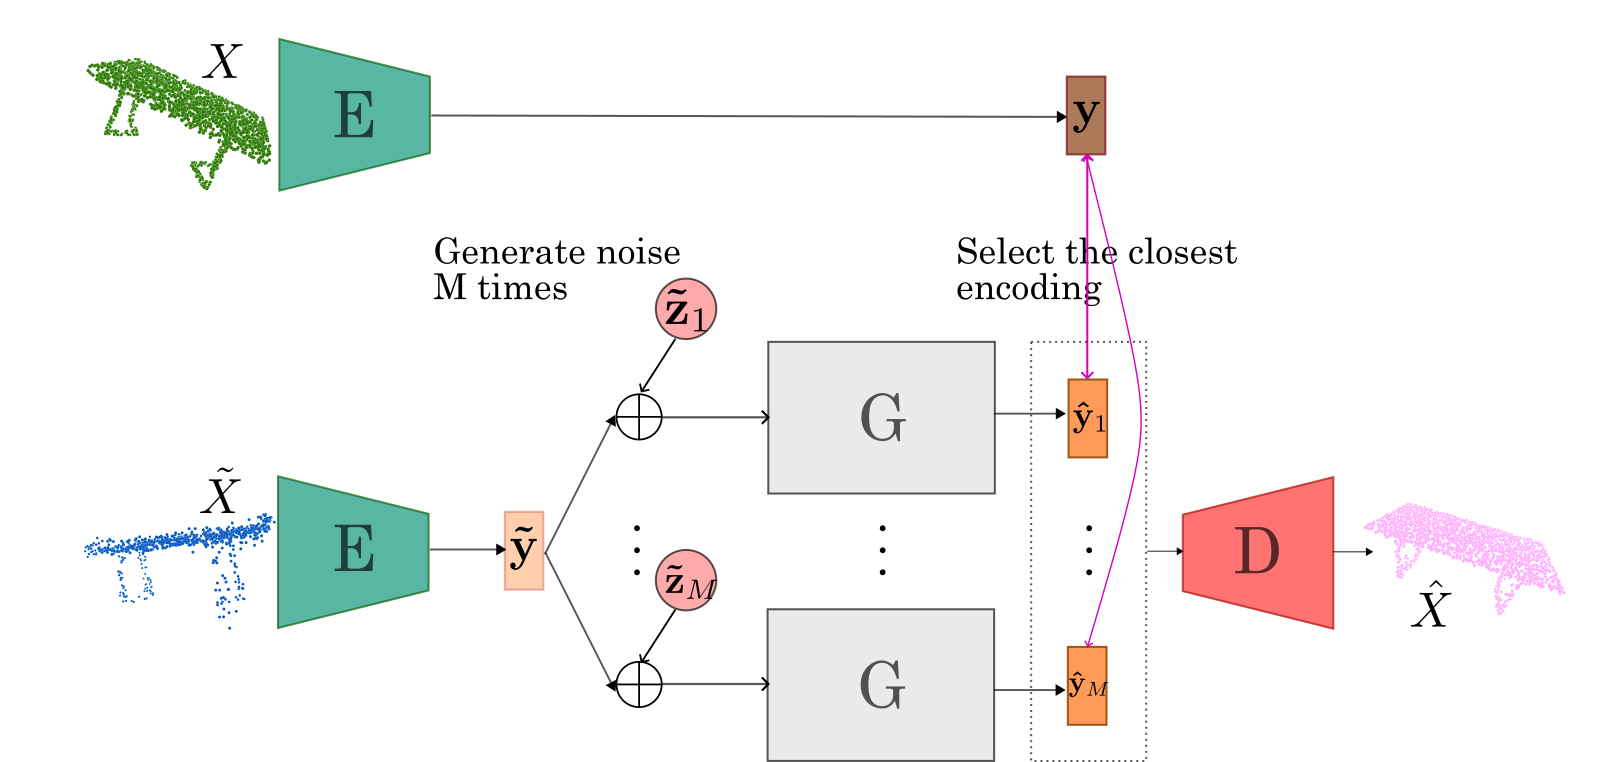
\includegraphics[width=\linewidth]{figures/implicit_gen_network_imle.png}
          \end{center}
          \caption{IMLE.}\label{fig:imle}
        \end{figure}
        Training differs according to the method selected for uncertainty quantification (more precisely, methods for inducing randomness) to produce different complete shapes. If we use dropout or DropConnect, the training procedure becomes quite straightforward. We follow the same general structure for point completion depicted in Figure~\ref{fig:gen_net} with the generator $G$ using dropout or DropConnect during training. If we use an ensemble of generators with $M$ models, then each generator needs to be trained individually, resulting in $M$ different training sequences similar to the procedure shown in Figure~\ref{fig:ens_net}. In this case, the inference and training follow the same pattern. 
        \newline
        
        Finally, for the implicit generation, we learn to produce different complete shapes for a fixed partial input based on the noise injected into the generator. Since only one possible target shape is available for each partial shape, we need to train it differently from just computing the loss based on the one-to-one correspondence. Otherwise, any addition of noise will be rendered inconsequential, resulting in mode collapse and similar completion results. Note that this is not an issue for dropout or ensemble models. With dropping out, the uncertainty is inherently induced through the different selection of weights or nodes during training. For the ensemble, we train all the models separately. 
        \\
        For training conditional implicit generative models, conditional Generative Adversarial Networks (GANs) had been the go-to approach for a long period. However, due to several drawbacks, such as mode collapse, the popularity of GANs has dwindled, with new approaches overturning the downsides of using GANs. One such method, called Implicit Maximum Likelihood Estimation (IMLE), was introduced by~\cite{IMLE}.~\cite{PCCIMLE} already applied the same idea for point cloud completion, which we adopt here.~\cite{PCCIMLE} showed that using conditional IMLE to train implicit generation results in more diverse completion results, resolving the mode collapse issue. Here, rather than comparing all the generated encodings ($\{\mathbf{\hat{y}}_i\}_{i=1}^M$) with the encoding of the complete shape $\mathbf{y}$, we only choose the one closest to $\mathbf{y}$ as shown in Figure~\ref{fig:imle}. This way, not every generated encoding is close to the encoding of the complete cloud, but every complete shape encoding has one generated encoding trained to be close in the latent space. This ensures that mode collapse does not happen, and every complete shape in the training data has at least one similar shape generated.

        \begin{figure}[htb]
          \begin{center}
          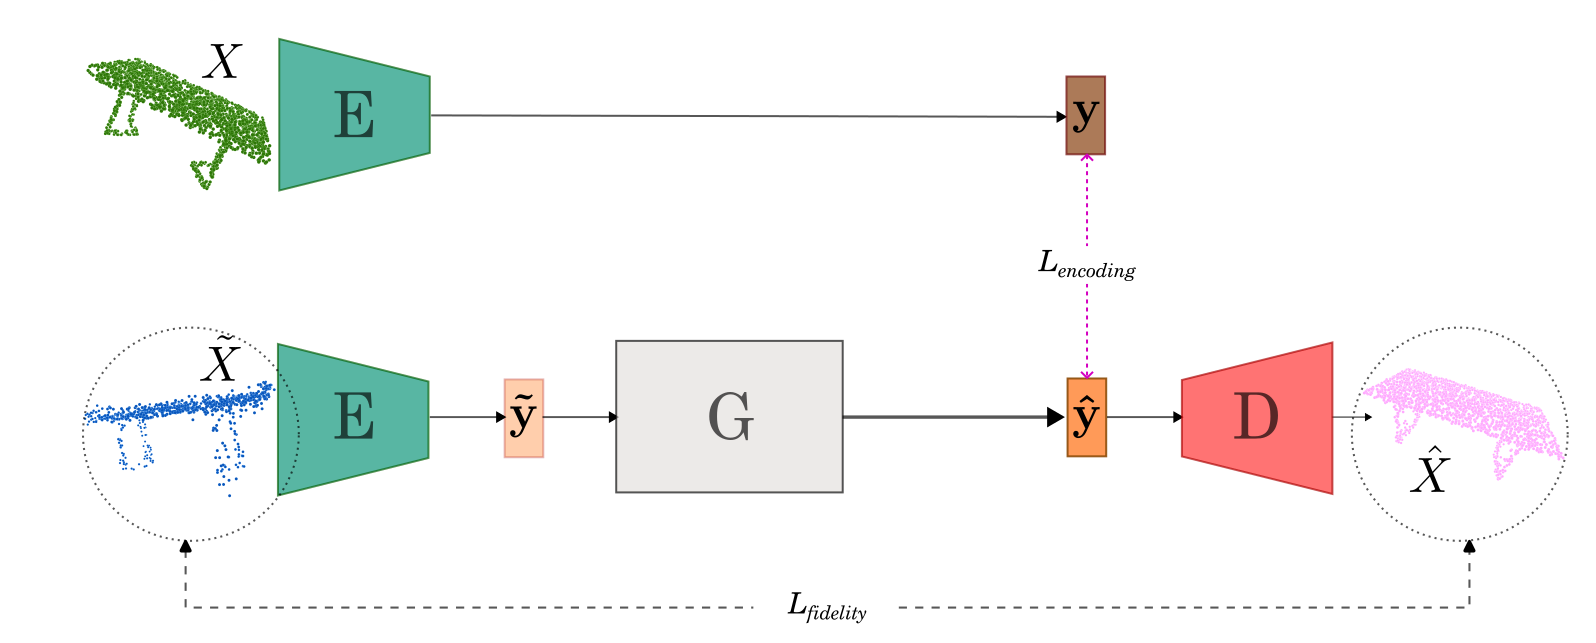
\includegraphics[width=\linewidth]{figures/losses_main_network.png}
          \end{center}
          \caption{Losses for training the main network for point cloud completion with uncertainty.}\label{fig:losses_main}
        \end{figure}
        To train the network (generator), we need to specify the loss functions we want to minimize (see Figure~\ref{fig:losses_main}). As discussed above, we fix the parameters of the encoder-decoder network trained for reconstruction. For a ground truth point cloud $X=\left\{\mathbf{x}_{i} \in \mathbb{R}^{3}\right\}_{i=1}^{N_C}$ from the dataset of complete clouds $\mathbf{X_C} \in \mathbb{R}^{N \times N_C \times 3}$, we pass it to the encoder network to get its encoding $\mathbf{y}$. Similarly, we feed the corresponding point cloud $\tilde{X}=\left\{\mathbf{\tilde{x}}_{i} \in \mathbb{R}^{3}\right\}_{i=1}^{N_P}$ from the dataset of partial clouds $\mathbf{X_P} \in \mathbb{R}^{N \times N_P \times 3}$ to obtain its encoding $\mathbf{\tilde{y}}$. Now we pass $\mathbf{\tilde{y}}$ through the generator according to the selected architecture among the ones explained above. For dropout or DropConnect, we generate only one encoding $\mathbf{\hat{y}}$ and compare it with $\mathbf{y}$. Otherwise, we generate $M$ encodings $\{\mathbf{\hat{y}}_i\}_{i=1}^M$ corresponding to the $i$-th model in the ensemble or $i$-th noise sampled for implicit generation. In the ensemble method, we compare each of $\{\mathbf{\hat{y}}_i\}_{i=1}^M$ to $\mathbf{y}$. In implicit generation, we follow the proposed IMLE method and compare the encoding in $\{\mathbf{\hat{y}}_i\}_{i=1}^M$ closest to $\mathbf{y}$ with $\mathbf{y}$. We denote the corresponding loss function between two encodings as:
        \begin{equation}\label{latent_loss}
            L_{encoding}(\mathbf{y}, \mathbf{\hat{y}}) = \left\|\mathbf{y} - \mathbf{\hat{y}}\right\|_2^2,
        \end{equation}
        which is the Euclidean distance between the two encodings. 
        \\
        We also need to ensure that the complete shapes generated are faithful to the partial shape. To maintain the fidelity of the completion results produced from the encodings output by the generator, we use the unidirectional Hausdorff distance between the partial cloud and the generated complete cloud. The corresponding loss is denoted as:
        \begin{equation}\label{fidelity_loss}
            L_{fidelity}(\tilde{X}, \hat{X}) = \max_{\mathbf{\tilde{x}}_{i} \in \tilde{X}} \min_{\mathbf{\hat{x}}_{j} \in \hat{X}} \left\|\mathbf{\tilde{x}}_{i}-\mathbf{\hat{x}}_{j}\right\|_2,
        \end{equation}
        where $\hat{X}=\left\{\mathbf{\hat{x}}_{j} \in \mathbb{R}^{3}\right\}_{j=1}^{N_C}$ is the set of generated point clouds. So the overall objective for training the network is:
        \begin{equation}\label{gen_obj}
            \begin{aligned}
                \mathcal{L}_{pcc} = \mathbb{E}_{X, \tilde{X} \sim p(X, \tilde{X})} \left[\lambda_{encoding} L_{encoding}\left(\mathcal{E}(X), \mathcal{G}_\theta(\mathcal{E}(\tilde{X}))\right)\right \\
                + \left\lambda_{fidelity} L_{fidelity}(\tilde{X}, \mathcal{D}\left(\mathcal{G}_\theta(\mathcal{E}(\tilde{X})))\right)\right]
            \end{aligned},
        \end{equation}
        where $\mathcal{E}$ is the encoder mapping, $\mathcal{D}$ is the decoder mapping, and $\mathcal{G}_\theta$ is the generator mapping by the NN parametrized by $\theta$. For IMLE, the above objective changes to:
        \begin{equation}\label{gen_obj_imle}
            \begin{aligned}
                \mathcal{L}_{pcc}^{imle} = \mathbb{E}_{X, \tilde{X} \sim p(X, \tilde{X}), \mathbf{Z}} \left[\lambda_{encoding} \min_{i=1, \ldots, M} L_{encoding}\left(\mathcal{E}(X), \mathcal{G}_\theta(\mathcal{E}(\tilde{X}), \mathbf{\tilde{z}}_i)\right)\right \\
                + \left\lambda_{fidelity} L_{fidelity}(\tilde{X}, \mathcal{D}\left(\mathcal{G}_\theta(\mathcal{E}(\tilde{X})))\right)\right]
            \end{aligned},
        \end{equation}
        where $\mathbf{Z} = (\mathbf{\tilde{z}}_1, \ldots, \mathbf{\tilde{z}}_M)^T$ such that $\mathbf{\tilde{z}}_i \sim \mathcal{N}(0, I_z) \forall i=\{1, \ldots, M\}$ with noise dimension $z$ and hyperparameter M.


    \subsection{Uncertainty Map Computation with Matching}
    Rather than naively computing the index-wise mean and variance of the 3D coordinates of the generated complete clouds, the point sets can be matched between themselves as one-to-one mappings of points. Such matchings between two point clouds can be computed using a minimum-weight matching or linear assignment with an appropriate cost of matching a point from one cloud to a point in another. Hungarian matching algorithm~\cite{Hungarian} or a modified version of Jonker-Volgenant algorithm~\cite{RectAssign} were applied to perform the matching between clouds. Euclidean distance between points was used as the cost function. One of the generated complete clouds we selected at random, and one-to-one mappings with points in the remaining complete clouds were identified. We then used the resulting matching to compute the mean and variance estimations of the predicted complete point cloud.


\section{Empirical Uncertainty Quantification for Implicit Neural Representation}\label{euqinr}
In this section, we propose to solve the Problems~\ref{SingleCloud} and~\ref{DataCloud} by predicting uncertain implicit representations for the given input cloud. An implicit representation is a function $f: \mathbb{R}^{3} \mapsto \mathbb{R}$ such that the zero level set of $f$ precisely approximates the surface on the 3D shape denoted by $\mathcal{S}$ :
\begin{equation}
\mathcal{S} \approx \left\{\mathbf{x} \in \mathbb{R}^{3} \mid f(\mathbf{x})=0\right\}
\end{equation}
\newline

Instead of directly computing the probabilistic estimate of the underlying surface, we first generate multiple possible implicit representations $\{f_i: \mathbb{R}^3 \mapsto \mathbb{R}\}_{i=1}^M$ from the input and then empirically estimate the surface along with the associated uncertainty from the different implicit representations. From previous works, we know that the neural implicit function $f$ usually approximates the (un-)signed distance function (UDF/SDF), which maps any point in space to the distance to its closest point on the surface. For a function $f$ to be a distance function corresponding to a given point cloud $X=\left\{\mathbf{x}_{i} \in \mathbb{R}^{3}\right\}_{i=1}^{N_C}$, it needs to satisfy some conditions or constraints as enumerated below~\cite{DiGS, NeuralHessian}:
\begin{enumerate}
    \item Dirichlet condition or manifold constraint: the observed points in the point cloud lie on the surface of the object, $f(\mathbf{x})=0$ for $\mathbf{x} \in X$.
    \item Eikonal constraint: all points have a unit gradient, $\|\nabla f\|=1$.
    \item Neumann condition or normal constraint:  the gradients of points match the ground truth normal field if normal information is available, $\nabla f=\mathcal{N}$, where $\mathcal{N}$ is the normal field.
    \item Non-manifold constraint: non-manifold points (points not on the surface) have the same value as their ground truth SDF or UDF if the distance values are available.
    \item Non-manifold penalisation constraint: non-manifold points have non-zero implicit function values.
\end{enumerate}
Out of the above constraints, while the manifold constraint and one of the Eikonal constraint or the Non-manifold constraint are necessary, the rest are mostly used as additional criteria to enhance the results~\cite{DiGS}. Since we are dealing with unoriented point clouds without normal information or SDF/UDF values for supervision, we cannot use normal and non-manifold constraints. We use the remaining 3 constraints for a given point cloud $X=\left\{\mathbf{x}_{i} \in \mathbb{R}^{3}\right\}_{i=1}^{N_C}$, which gives us the following loss functions:
\begin{equation}\label{manifold_sdf}
    \mathcal{L}_{\text {manifold }}=\int_{X}\|f(x)\|_{1} d x \approx \frac{1}{N_C}\sum_{i=1}^{N_C}\|f(\mathbf{x}_i)\|_1
\end{equation}
\begin{equation}\label{non_manifold_sdf}
    \mathcal{L}_{\text {non-manifold }}=\int_{\underline{X}} \exp \left(-\alpha\|f(x)\|_{1}\right) d x \approx \frac{1}{N_C}\sum_{i=1}^{N_C} \exp \left(-\alpha\|f(\underline{\mathbf{x}_i})\|_1\right),
\end{equation}
where $\underline{X}=\left\{\underline{\mathbf{x}_i} \in \mathbb{R}^{3}\right\}_{i=1}^{N_C}$ is the set of points off the surface and $\alpha>>1$.
\begin{equation}\label{Eikonal}
     \begin{aligned}
         \mathcal{L}_{\text {Eikonal }}=\int_{X \cup \underline{X}} \| \| \nabla f(x)\left\|_{2}-1\right\|_{1} d x \\
         \approx \frac{1}{N_C}\sum_{i=1}^{N_C} \left(\| \| \nabla f(\mathbf{x}_i)\left\|_{2}-1\right\|_{1} + \| \| \nabla f(\underline{\mathbf{x}_i})\left\|_{2}-1\right\|_{1} \right).
     \end{aligned}
\end{equation}
We can then compute the combined objective function as:
\begin{equation}\label{inr_loss1}
    \mathcal{L}_{inr}= \lambda_{\text {manifold }} \mathcal{L}_{\text {manifold }}+\lambda_{\text {non-manifold }} \mathcal{L}_{\text {non-manifold }}+ \lambda_{\text {Eikonal }} \mathcal{L}_{\text {Eikonal }}
\end{equation}
where $\lambda_{\text {manifold }}, \lambda_{\text {non-manifold }}, \lambda_{\text {Eikonal }}$ are the corresponding regularization weights.
\newline

However, optimizing the above objective is not sufficient to produce optimal results, as demonstrated by~\cite{DiGS, NeuralHessian}. As discussed in section~\ref{INR-old}, several works have tried to solve this issue by introducing an additional loss depending upon the intended geometric effect. Since we are working with unoriented point clouds, we will employ the loss based on the Hessian matrix defined in~\cite{NeuralHessian}. The loss function associated with the Hessian matrix can be computed as:
\begin{equation}\label{Hessian1}
    \mathcal{L}_{\text{Hessian }} = \int_{\circled{$X$}} \left|Det(\mathbf{H}_f(x))\right| d x \approx \frac{1}{N_C}\sum_{i=1}^{N_C} \left|Det\left(\mathbf{H}_f\left(\circled{$\mathbf{x}_i$}\right)\right)\right|,
\end{equation}
where $\circled{$X$}=\left\{\circled{$\mathbf{x}_i$} \in \mathbb{R}^{3}\right\}_{i=1}^{N_C}$ is the set of points close to the surface and $Det(\cdot)$ refers to the determinant of the matrix. So the overall objective function now becomes:
\begin{equation}\label{Hessian2}
    \mathcal{L}_{inr}= \lambda_{\text {manifold }} \mathcal{L}_{\text {manifold }}+\lambda_{\text {non-manifold }} \mathcal{L}_{\text {non-manifold }}+ \lambda_{\text {Eikonal }} \mathcal{L}_{\text {Eikonal }}+ \lambda_{\text{Hessian }} \tau \mathcal{L}_{\text{Hessian }},
\end{equation}
where $\tau$ is the annealing factor defined in~\cite{NeuralHessian}. Now with the objective defined, we can discuss introducing randomness in our implicit function prediction to calculate uncertainty.


    \subsection{Predicting Implicit Representation with Randomness}
    \begin{figure}[htb]
      \begin{center}
      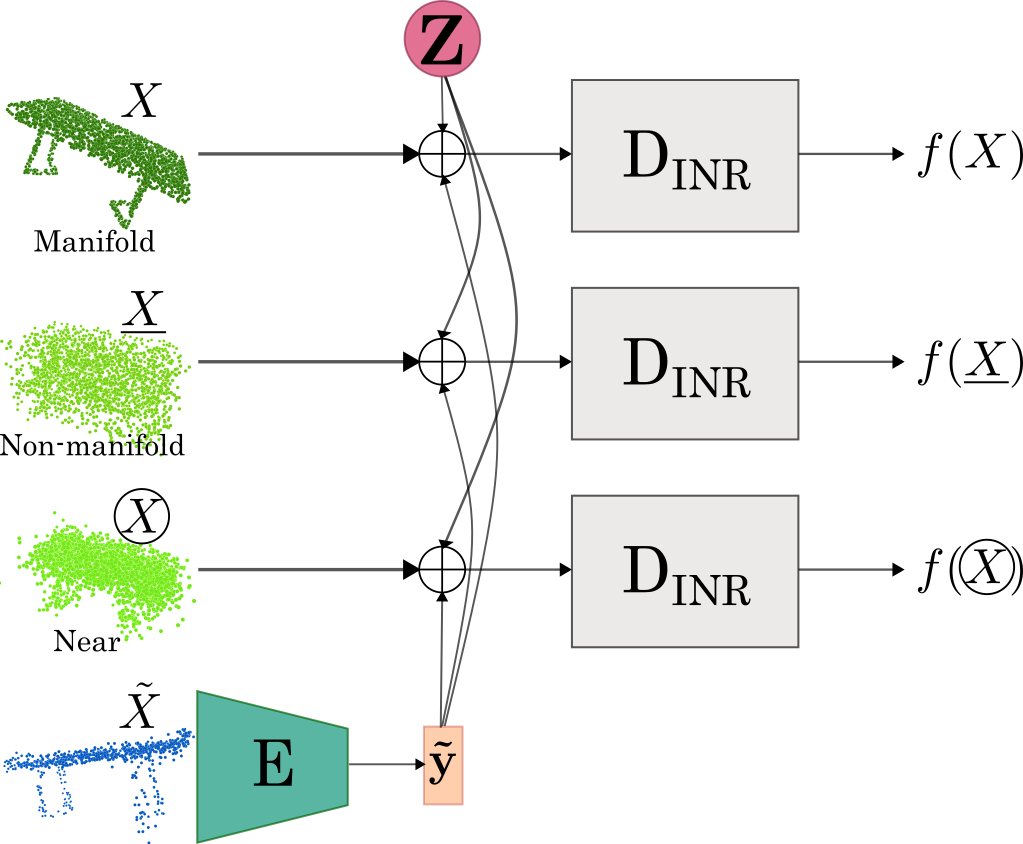
\includegraphics[width=\linewidth]{figures/inr_network.png}
      \end{center}
      \caption{General structure of network used for training implicit function with randomness. During training, the partial cloud $\tilde{X}$ is input to the encoder E to output the encoding $\mathbf{\tilde{y}}$. Manifold, non-manifold, and near points conditioned on $\mathbf{\tilde{y}}$ and noises are fed to the decoder D$_{\text{INR}}$ to predict the implicit function corresponding to the noise.}\label{fig:inr_net}
    \end{figure}
    We can introduce randomness in the network architecture that approximates the implicit function utilizing any of the uncertainty quantification methods discussed in section~\ref{back_uqdl}. For Problem~\ref{SingleCloud}, the network structure is straightforward. We can use existing shape space learning architectures for point clouds, such as a standard or variational auto-encoder, with the decoder output being the implicit representation instead of a reconstructed cloud. On the other hand, for Problem~\ref{DataCloud}, during training, we have access to partial and complete cloud pairs but only the partial cloud for inference. So, we will have an information disparity between the training and inference processes if we directly learn the implicit representation from complete clouds in the shape space. To get a clearer picture regarding the information lost without the complete cloud, we first describe the sampling procedure used to learn the implicit function.
    \newline
    
    To sample points not on the surface (points in the set $\underline{X}$), we find a bounding box around the point cloud and uniformly sample points within that box. Considering most points inside the box are off the surface, sampling a point on the surface is highly unlikely. To sample points close to the surface (points in the set \circled{$X$}), we emulate the sampling used in~\cite{IGR, SALD, NeuralHessian}. For each point $\mathbf{x}_i$ on the surface, we find the distance to the $k$-th nearest point ($k=50$ used by previous methods) as $d$. Then we sample one point from the Gaussian distribution $\mathcal{N}(\mathbf{x}_i, d^2I)$ to find a point close to the surface. We observe that while sampling of non-manifold points is not affected by the unavailability of a complete cloud, sampling of points close to the surface differs. So, we avoid using points close to the surface during inference. Also, since at test time, only the partial point cloud is available, we can't use encoding of the complete cloud while learning. With all that in mind, we propose the architecture depicted in Figure~\ref{fig:inr_net}.
    \newline
    
    We consider the complete point cloud $X$ as the points lying on the surface (manifold points). We sample the non-manifold and near point sets $\underline{X}$ and \circled{$X$} as explained. We feed the partial cloud $\tilde{X}$ to the encoder E to get the encoding $\mathbf{\tilde{y}}$. Parallelly, we sample multiple noises $\mathbf{Z} = (\mathbf{\tilde{z}}_1, \ldots, \mathbf{\tilde{z}}_M)^T$ such that $\mathbf{\tilde{z}}_i \sim \mathcal{N}(0, I_z) \forall i=\{1, \ldots, M\}$ with noise dimension $z$ and hyperparameter M. We then pass the manifold, non-manifold, and near points conditioned on the encoding $\mathbf{\tilde{y}}$ and noises to the decoder D$_{\text{INR}}$ to predict the implicit function corresponding to each noise. If we train to minimize the objective for the implicit function predicted for each noise, we might run into the issue of mode collapse. This will lead to a lack of diversity in predicted implicit functions. Therefore, during training, we only choose the noise leading to the implicit function with minimum manifold loss ($\mathcal{L}_{\text {manifold }}$) for computing the rest of the objective function and performing backpropagation. During inference, we predict different implicit functions based on different noises and empirically estimate the mean and variance at any point based on those predicted functions to obtain our reconstructed surface with associated uncertainty.
    \newline
    
    We also need to regularize our learned encoding for better shape space learning using autoencoder architectures. For a standard autoencoder, the regularization loss can be computed as:
    \begin{equation}\label{reg_latent}
        \mathcal{L}_{\text {reg }} = \left\|\mathcal{E}(\tilde{X})\right\|_2^2,
    \end{equation}
    where $\mathcal{E}$ is the encoder mapping. For a variational autoencoder, the  regularization loss can be computed as (similar to~\cite{SAL}):
    \begin{equation}\label{reg_latent}
        \mathcal{L}_{\text {reg }} = \left\|\mu\left(\mathcal{E}(\tilde{X})\right)\right\|_1 +\left\|diag(\Sigma\left(\mathcal{E}(\tilde{X})\right)\right\|_1,
    \end{equation}
    where $diag$ is the diagonal matrix, $\mu$ denotes the latent prediction (mean function) and $\Sigma$ refers to the covariance matrix for latent prediction. Such regularization enforces the latent means to be near zero and the covariances to be close to identity matrices. With the addition of the regularization term, the overall objective function becomes:
    \begin{equation}\label{Hessian3}
        \mathcal{L}_{inr}= \lambda_{\text {manifold }} \mathcal{L}_{\text {manifold }}+\lambda_{\text {non-manifold }} \mathcal{L}_{\text {non-manifold }}+ \lambda_{\text {Eikonal }} \mathcal{L}_{\text {Eikonal }}+ \lambda_{\text{Hessian }} \tau \mathcal{L}_{\text{Hessian }} + \lambda_{\text {reg }} \mathcal{L}_{\text {reg }},
    \end{equation}

    

\section{Gaussian Process-based Uncertainty Quantification for 3D Shapes}\label{gpuq}
In this section, we try to tackle the Problems~\ref{SingleCloud} and~\ref{DataCloud} by describing an uncertain implicit representation for the given input cloud by a Gaussian process. There are several existing works (see section~\ref{Stoch-old}) that followed a similar approach for a single point cloud (Problem~\ref{SingleCloud}). So, we will only focus on methods to solve Problem~\ref{DataCloud}.

\begin{figure}[htb]
      \begin{center}
      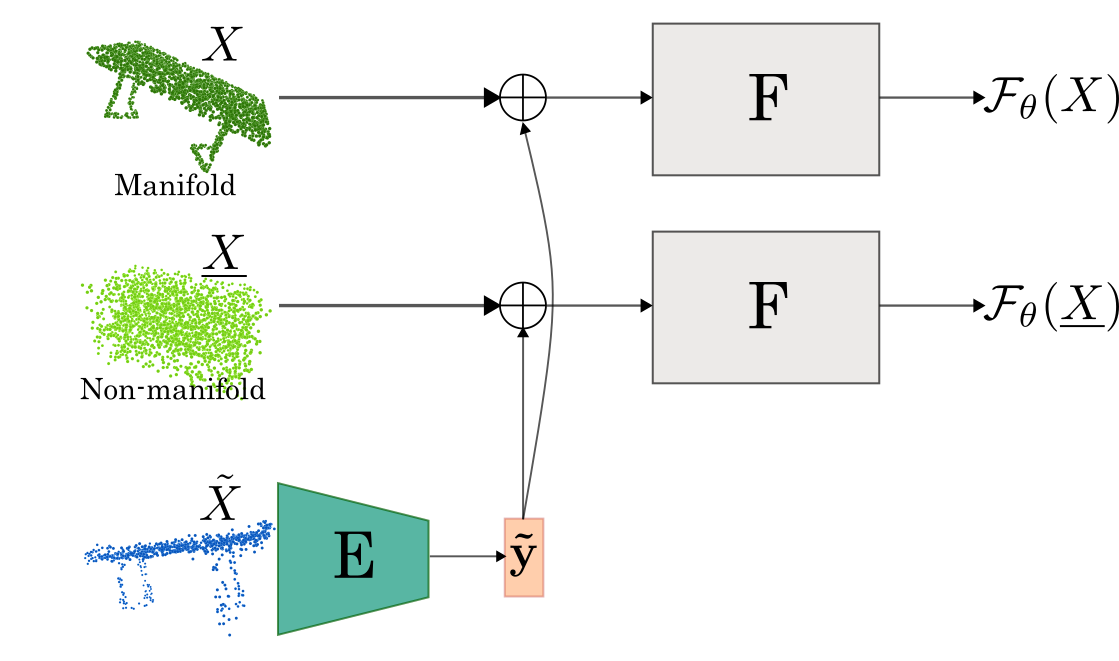
\includegraphics[width=\linewidth]{figures/gpr_network.png}
      \end{center}
      \caption{General structure of network used for learning feature mapping. During training, the partial cloud $\tilde{X}$ is input to the encoder E to output the encoding $\mathbf{\tilde{y}}$. Manifold and non-manifold points conditioned on $\mathbf{\tilde{y}}$ are fed to the neural network F to predict the output of feature mapping $\mathcal{F}_\theta$.}\label{fig:gpr_net}
\end{figure}

We know that the surface is represented by the zero level set of the implicit function $f: \mathbb{R}^{3} \mapsto \mathbb{R}$. Therefore, for all non-manifold points $\mathbf{x} \in \mathbb{R}^{3}$, $f(\mathbf{x}) \neq 0$. For a given partial and complete cloud pair, we want to learn a function that outputs zero for points on the surface and non-zero values otherwise when conditioned on the partial point cloud. Similar to the method described in section~\ref{euqinr}, we encode the partial cloud $\tilde{X}$ to get the latent code $\mathbf{\tilde{y}}$. We consider the complete point cloud $X$ as the points lying on the surface (manifold points). As in section~\ref{euqinr}, we sample non-manifold points by finding a bounding box around the complete cloud and uniformly sampling points within that box. Now, we want the Gaussian process posterior mean for each manifold point conditioned on $\mathbf{\tilde{y}}$ to be zero, and for non-manifold points conditioned on $\mathbf{\tilde{y}}$ farther from zero.
\newline

Another aspect to consider is that we have only observed unoriented point clouds, meaning we only have samples $\mathbf{x}$ for which $f_{\mathbf{\tilde{y}}}(\mathbf{x}) = 0$ where $f_{\mathbf{\tilde{y}}}$ denotes the implicit function $f$ conditioned on the encoding $\mathbf{\tilde{y}}$ of partial cloud. Although we sampled points off the surface, we don't know their ground truth function value. This makes the problem quite challenging since, without supervision from non-zero valued samples, the Gaussian process regression fails to predict non-zero values for the points not on the surface, leading to multiple ghost geometries. This is also evident from Eq.~\ref{GPPosterior} as the posterior mean becomes zero if $\mathbf{Y}=\mathbf{0}$. 



%%%%%%%%%%%%%%%%%%%%%%%%%%%%%%%%%%%%%%%%%%%%%%%%%%%%%%%%%%%%%%%%%%%%%%%%%%%%%%%%%%%%%%%%%%%%%%%%%%%%%